
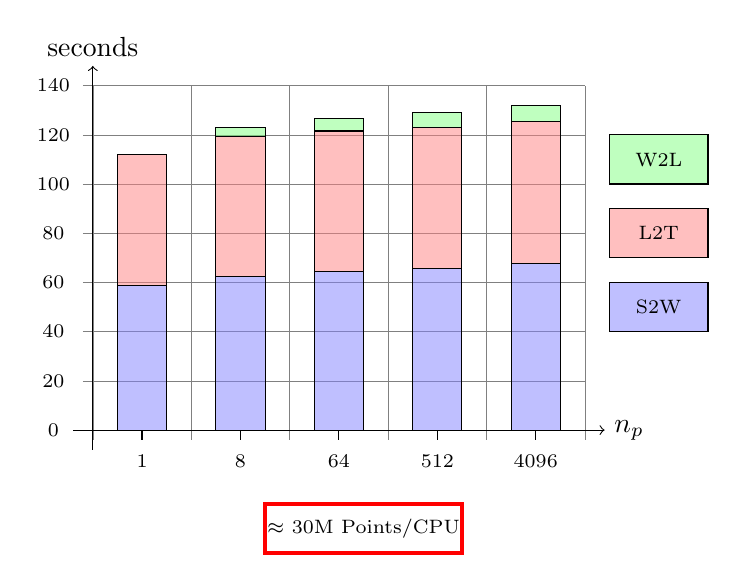
\begin{tikzpicture}[scale=1.25]

\draw[very thin, color=gray, xstep=1, ystep=0.5] (-0.1,-0.1) grid (5, 3.5);
\draw[->] (-0.2, 0) -- (5.2, 0) node[right] {$n_p$};
\draw[->] (0, -0.2) -- (0, 3.7) node[above] {seconds};

\newdimen\yscale

\yscale= 0.025 cm

\foreach \pos/\label in {0.5/1, 1.5/8, 2.5/64, 3.5/512, 4.5/4096} {
\draw (\pos,0) -- (\pos,-0.1) (\pos cm,-2.5ex) node [anchor=base,fill=white,inner sep=1pt]  {\scriptsize{\label}};
}

\foreach \label in {0, 20, ..., 140} {
 \draw (-0.4, \label\yscale) node {\scriptsize{\label}};
}

\draw[fill=blue!50, fill opacity=0.5] (4.5, 2.25) ++ (0.75, -1.25) rectangle +(1.0, 0.5);
\draw (4.5, 2.25) ++ (1.25, -1.0) node {\scriptsize{S2W}};

\draw[fill=red!50, fill opacity=0.5] (4.5, 1.75) ++ (0.75, 0.0) rectangle +(1.0, 0.5);
\draw (4.5, 1.75) ++ (1.25, 0.25) node {\scriptsize{L2T}};

\draw[fill=green!50, fill opacity=0.5] (4.5, 1.25) ++ (0.75, 1.25) rectangle +(1.0, 0.5);
\draw (4.5, 1.25) ++ (1.25, 1.5) node {\scriptsize{W2L}};

\draw[red, ultra thick] (1.75, -1.25) rectangle +(2.0, 0.5);
\draw (2.75, -1.0) node {\scriptsize{$\approx$ 30M Points/CPU}};

\newdimen\mypos
\newdimen\myoff

\foreach \pos/\vala/\valb/\valc/\vald/\vale/\valf in { 
0/58.75/53.36/0.0698/112.19/29.2M/$\frac{1}{16}$,
1/62.25/56.98/3.90/120.93/233.8M/$\frac{1}{64}$,
2/64.39/57.18/4.93/125.06/1.9B/$\frac{1}{256}$,
3/65.56/57.50/5.92/127.62/15.0B/$\frac{1}{1024}$,
4/67.53/57.75/6.59/131.65/119.7B/$\frac{1}{4096}$ } { 

\mypos=\pos cm
\advance \mypos by 0.5 cm

\advance \mypos by -0.25 cm

\myoff=0 cm

\draw[fill=blue!50, fill opacity=0.5] (\mypos, \myoff) rectangle +(0.5, \vala\yscale);
\advance \myoff by \vala\yscale

\draw[fill=red!50, fill opacity=0.5] (\mypos, \myoff) rectangle +(0.5, \valb\yscale);
\advance \myoff by \valb\yscale

\draw[fill=green!50, fill opacity=0.5] (\mypos, \myoff) rectangle +(0.5, \valc\yscale);

}

\end{tikzpicture}

